\documentclass[border={0cm 0cm 0cm 0cm}]{standalone}  %E,S,W,N

\usepackage{amssymb,amsmath}
\usepackage{tikz}

\begin{document}
	
	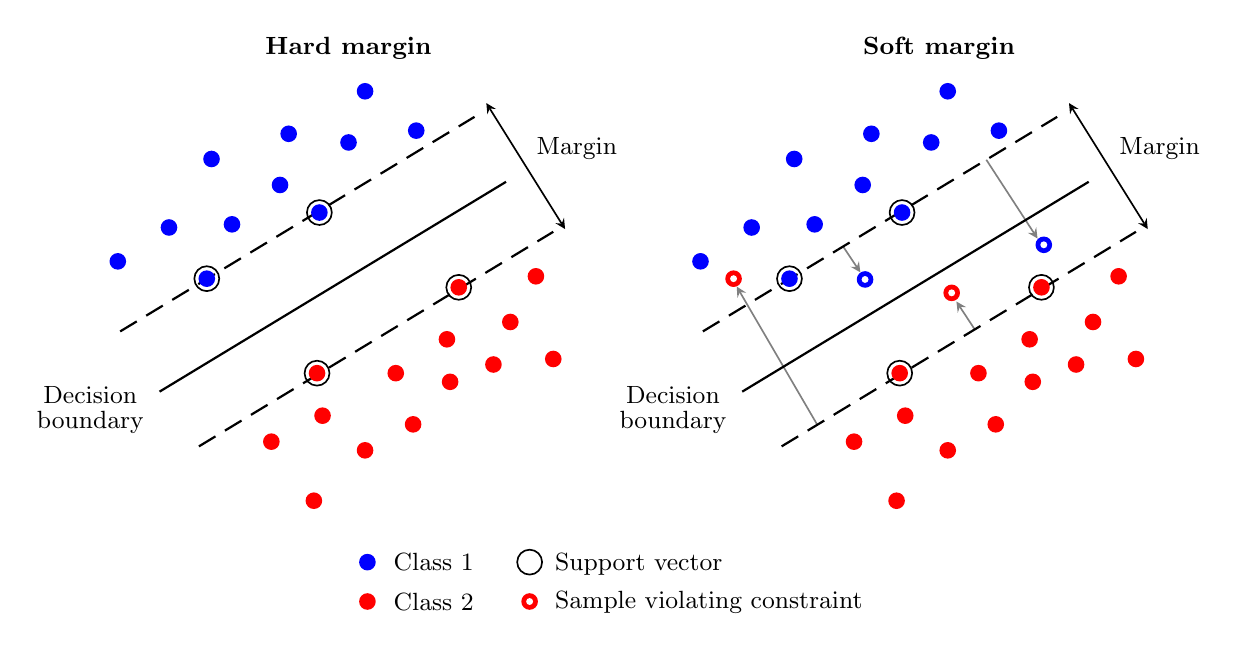
\begin{tikzpicture}	
	%DIFFERENCES BETWEEN VERSIONS
	\node at (4.1,7.7) {\bfseries\small Hard margin};
	\node at (4.1+7.5,7.7) {\bfseries\small Soft margin};
	\draw[semithick,gray,->,>=stealth] (2.55+7.5,2.92)--(1.53+7.5,4.67);
	\draw[semithick,gray,->,>=stealth] (2.88+7.5,5.18)--(3.1+7.5,4.85);
	\draw[semithick,gray,->,>=stealth] (4.55+7.5,4.13)--(4.32+7.5,4.48);
	\draw[semithick,gray,->,>=stealth] (4.7+7.5,6.28)--(5.35+7.5,5.28);
	%
	\fill[red] (1.49+7.5,4.77) circle (3pt);	\fill[white] (1.49+7.5,4.77) circle (1.25pt);
	\fill[red] (4.26+7.5,4.59) circle (3pt);	\fill[white] (4.26+7.5,4.59) circle (1.25pt);
	\fill[blue] (3.16+7.5,4.76) circle (3pt);	\fill[white] (3.16+7.5,4.76) circle (1.25pt);
	\fill[blue] (5.43+7.5,5.2) circle (3pt);	\fill[white] (5.43+7.5,5.2) circle (1.25pt);
	
	%LINES & LABELS
	\foreach \c in {0,7.4}{
	\node[align=center] at (0.82+\c,3.1) {\small Decision \\[-1mm] \small boundary};
	\draw[thick] (1.7+\c,3.335)--(6.1+\c,6);
	\draw[thick,dash pattern=on 7pt off 4pt] (1.2+\c,4.1)--(5.7+\c,6.825);
	\draw[thick,dash pattern=on 7pt off 4pt] (2.2+\c,2.64)--(6.7+\c,5.365);
	\draw[semithick,<->,>=stealth] (6.85+\c,5.4)--(5.85+\c,7);
	\node at (7+\c,6.42) {\small Margin};
	
	%DOTS -- BLUE
	\fill[blue] (1.17+\c,4.99) circle (3pt);
	\fill[blue] (2.3+\c,4.77) circle (3pt);		\draw[semithick] (2.3+\c,4.77) circle (4.5pt);
	\fill[blue] (1.82+\c,5.42) circle (3pt);
	\fill[blue] (2.36+\c,6.29) circle (3pt);
	\fill[blue] (2.62+\c,5.46) circle (3pt);
	\fill[blue] (3.23+\c,5.96) circle (3pt);
	\fill[blue] (3.34+\c,6.61) circle (3pt);
	\fill[blue] (3.73+\c,5.61) circle (3pt);	\draw[semithick] (3.73+\c,5.61) circle (4.5pt);
	\fill[blue] (4.1+\c,6.5) circle (3pt);
	\fill[blue] (4.31+\c,7.15) circle (3pt);
	\fill[blue] (4.96+\c,6.65) circle (3pt);
	
	%DOTS -- RED
	\fill[red] (3.12+\c,2.7) circle (3pt);
	\fill[red] (3.66+\c,1.95) circle (3pt);
	\fill[red] (3.77+\c,3.03) circle (3pt);
	\fill[red] (3.7+\c,3.57) circle (3pt);	\draw[semithick] (3.7+\c,3.57) circle (4.5pt);
	\fill[red] (4.31+\c,2.59) circle (3pt);
	\fill[red] (4.92+\c,2.92) circle (3pt);
	\fill[red] (4.7+\c,3.57) circle (3pt);
	\fill[red] (5.39+\c,3.46) circle (3pt);
	\fill[red] (5.35+\c,4) circle (3pt);
	\fill[red] (5.5+\c,4.66) circle (3pt);	\draw[semithick] (5.5+\c,4.66) circle (4.5pt);
	\fill[red] (5.94+\c,3.68) circle (3pt);
	\fill[red] (6.155+\c,4.22) circle (3pt);
	\fill[red] (6.48+\c,4.8) circle (3pt);
	\fill[red] (6.7+\c,3.75) circle (3pt);
		} %end foreach

	%LEGEND
	\fill[blue] (4.34,1.17) circle (3pt);
		\node[align=left,right] at (4.35+0.2,1.17) {\small Class 1};
	\fill[red] (4.34,0.67) circle (3pt);
		\node[align=left,right] at (4.35+0.2,0.67) {\small Class 2};
	\draw[semithick] (6.4,1.17) circle (4.5pt);
		\node[align=left,right] at (6.4+0.2,1.14) {\small Support vector};
	\fill[red] (6.4,0.67) circle (3pt);		\fill[white] (6.4,0.67) circle (1.25pt);
		\node[align=left,right] at (6.4+0.2,0.66) {\small Sample violating constraint};
	
	%\draw[help lines] (0,0) grid (14,8);
	\end{tikzpicture}
	
\end{document}